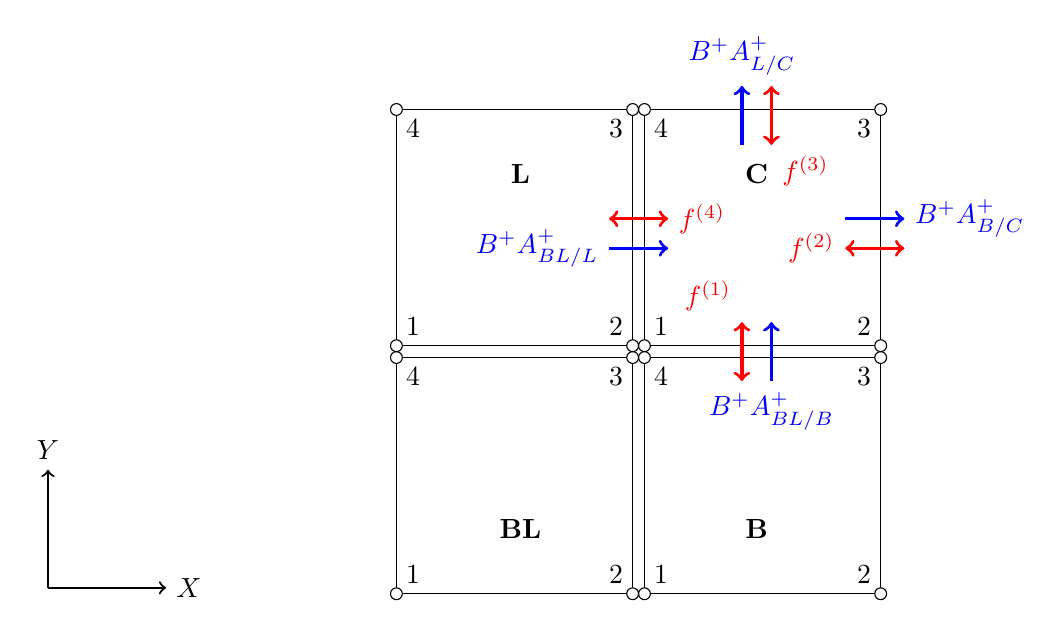
\begin{tikzpicture}[scale=1.5]
  \draw[thick,->] (-3,0.)-- (-2,0.) node[right] {$X$};
  \draw[thick,->] (-3,0.)-- (-3,1.) node[above] {$Y$};

  %% Cells
  \draw (0-0.05,0-0.05) rectangle (2.-0.05,2-0.05);
  \draw (0-0.05,2+0.05) rectangle (2.-0.05,4+0.05);
  \draw (2+0.05,0-0.05) rectangle (4.+0.05,2-0.05);
  \draw (2+0.05,2+0.05) rectangle (4.+0.05,4+0.05);
  %%%%%%%%%%%%%%%%%%%%%
  
  %% Nodes
  \fill[white] (0-0.05,0-0.05) circle (0.05);\fill[white] (2-0.05,2-0.05) circle (0.05);
  \fill[white] (0-0.05,2+0.05) circle (0.05);\fill[white] (2.-0.05,4+0.05) circle (0.05);
  \fill[white] (2+0.05,0-0.05) circle (0.05);\fill[white] (4.+0.05,2-0.05) circle (0.05);
  \fill[white] (2+0.05,2+0.05) circle (0.05);\fill[white] (4.+0.05,4+0.05) circle (0.05);
  \fill[white] (2-0.05,0-0.05) circle (0.05);\fill[white] (4.+0.05,0-0.05) circle (0.05);
  \fill[white] (0-0.05,2-0.05) circle (0.05);\fill[white] (2.+0.05,2-0.05) circle (0.05);
  \fill[white] (2-0.05,2+0.05) circle (0.05);\fill[white] (4.+0.05,2.+0.05) circle (0.05);
  \fill[white] (-0.05,4+0.05) circle (0.05);\fill[white] (2.+0.05,4+0.05) circle (0.05);

  \draw (0-0.05,0-0.05) circle (0.05) node[above right] {$1$};\draw (2-0.05,2-0.05) circle (0.05) node[below left] {$3$};
  \draw (0-0.05,2+0.05) circle (0.05) node[above right] {$1$};\draw (2.-0.05,4+0.05) circle (0.05) node[below left] {$3$};
  \draw (2+0.05,0-0.05) circle (0.05) node[above right] {$1$};\draw (4.+0.05,2-0.05) circle (0.05) node[below left] {$3$};
  \draw (2+0.05,2+0.05) circle (0.05) node[above right] {$1$};\draw (4.+0.05,4+0.05) circle (0.05) node[below left] {$3$};
  \draw (2-0.05,0-0.05) circle (0.05) node[above left] {$2$};\draw (4.+0.05,0-0.05) circle (0.05) node[above left] {$2$};
  \draw (0-0.05,2-0.05) circle (0.05) node[below right] {$4$};\draw (2.+0.05,2-0.05) circle (0.05) node[below right] {$4$};
  \draw (2-0.05,2+0.05) circle (0.05) node[above left] {$2$};\draw (4.+0.05,2.+0.05) circle (0.05) node[above left] {$2$};
  \draw (-0.05,4+0.05) circle (0.05) node[below right] {$4$};\draw (2.+0.05,4+0.05) circle (0.05) node[below right] {$4$};
  %%%%%%%%%%%%%%%%%%%%%%%

  %% Cells names
  \node at (3,3.5) {$\textbf{C}$};
  \node at (1,0.5) {$\textbf{BL}$};
  \node at (3,0.5) {$\textbf{B}$};
  \node at (1,3.5) {$\textbf{L}$};

  %% Transverse corrections
  \draw[->, very thick,Blue] (2.875,3.75) -- (2.875,4.25) node [above] {$B^+A^+_{L/C}$}; % Top
  \draw[->, very thick,Blue] (3.75,3.125) -- (4.25,3.125) node [right] {$B^+A^+_{B/C}$}; % Right
  \draw[<-, very thick,Blue] (3.125,2.25) -- (3.125,1.75) node [below] {$B^+A^+_{BL/B}$}; % Bottom
  \draw[<-, very thick,Blue] (2.25,2.875) -- (1.75,2.875) node [left] {$B^+A^+_{BL/L}$}; % Left

  %% Normal fluxes
  \draw[<->, very thick,Red] (3.125,3.75) node [below right] {$f^{(3)}$} -- (3.125,4.25) ; % Top
  \draw[<->, very thick,Red] (3.75,2.875) node [left] {$f^{(2)}$}-- (4.25,2.875) ; % Right
  \draw[<->, very thick,Red] (2.875,2.25) node [above left] {$f^{(1)}$}-- (2.875,1.75); % Bottom
  \draw[<->, very thick,Red] (2.25,3.125) node [right] {$f^{(4)}$} -- (1.75,3.125); % Left

  % %% Edges numbers
  % \node[above] at (1,-0.1) {$(1)$};
  % \node[left] at (2,1.) {$(2)$};
  % \node[below] at (1,1.95) {$(3)$};
  % \node[right] at (-0.1,1.) {$(4)$};
\end{tikzpicture}


%%% Local Variables:
%%% mode: latex
%%% TeX-master: "../../mainManuscript"
%%% End:
